\chapter{Bipolar Junction Transistor}\label{chap3}

The first Junction transistor\index{Transistor} was invented in 1947 at the Bell Telephone Laboratories by Dr. William Schockley and his co-inventors Dr. John Bardeen and Dr. Brattain. Transistor is capable of amplifying electronic signals such as radio and TV signals.

This chapter discusses the construction of Bipolar Junction Transistor (BJT), its working and its characteristics. The amplification property of BJT and its configurations are also discussed.

\section{Transistor construction}\label{sec3.1}
\index{Transistor!construction}\index{Bipolar Junction Transistor!construction}

The Bipolar Junction Transistor\index{Bipolar Junction Transistor} or simply transistor is a three layer two junction semiconductor device consisting of either two $n$ and one $p$-type layers of material or two $p$ and one $n$-type layers of material. The former is called an $npn$ transistor, while the latter is called a $pnp$ transistor.
Fig.~\ref{fig3.1}(a) shows the construction of an $npn$ transistor.\index{npn@$npn$ transistor}\index{Transistor!npn@$npn$ transistor}
\begin{figure}[H]
\centering
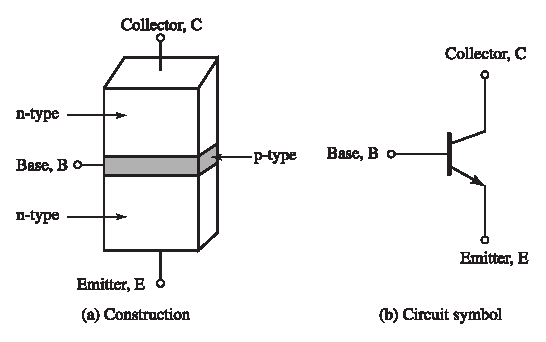
\includegraphics[scale=.93]{chap2/S3-EE-03-001.eps}
\caption{$npn$ transistor}\label{fig3.1}
\end{figure}

\vfill\eject

The three layers of the transistor are named as emitter $(E)$, base $(B)$ and collector $(C)$. The emitter layer is heavily doped, the base lightly doped, and the collector is moderately doped. The outer layers (Emitter and Collector) have widths much greater than the middle layer (base), typically $10:1$.

Fig.~\ref{fig3.1}(b) shows the circuit symbol of $npn$ transistor. Note that the emitter current is shown flowing out of emitter terminal.

The construction\index{pnp@$pnp$ transistor!construction} and circuit symbol of a $pnp$ transistor\index{pnp@$pnp$ transistor}\index{Transistor!pnp@$pnp$ transistor} are shown in Fig.~\ref{fig3.2}.
\begin{figure}[H]
\centering
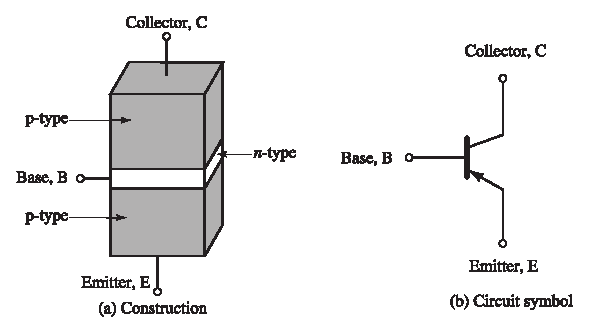
\includegraphics{chap2/S3-EE-03-002.eps}
\caption{$pnp$ transistor}\label{fig3.2}
\end{figure}

Observe that, the emitter current direction in $pnp$ transistor is shown flowing into the emitter terminal. The arrow on emitter terminal indicates the conventional direction of current flow.

The term bipolar in BJT reflects the fact that both holes and electrons contribute to the flow of current in a transistor.

\section[Barrier voltages in unbiased $npn$ transistor]{Barrier voltages in unbiased \boldmath$npn$ transistor}\label{sec3.2}

Fig.~\ref{fig3.3} shows the depletion regions\index{Depletion regions} and barrier voltages\index{npn@$npn$ transistor!barrier voltages} in an unbiased $npn$ transistor.

\vskip .1cm

Depletion region is a region where there are no free charges. The middle layer is very thin compared to the outer layers. Also the outer layers are also much more heavily doped than the center layer. As a result the depletion regions\index{npn@$npn$ transistor!depletion regions} penetrate deep into the base, from either side.

\vskip .1cm

Because of this penetration, the distance between the two depletion layers, within the base, is very short. Observe that the junction barrier voltages are positive on the emitter and collector, and negative on the base of the $npn$ device.
\begin{figure}[H]
\centering
\includegraphics{chap2/S3-EE-03-003.eps}
\caption{Depletion regions and barrier voltages in an unbiased $npn$ transistor}\label{fig3.3}
\end{figure}


\section[Operation of $npn$ transistor]{Operation of \boldmath$npn$ transistor}\label{sec3.3}
\index{npn@$npn$ transistor!operation of}

Fig.~\ref{fig3.4} shows an $npn$ transistor with external bias voltages.
\begin{figure}[H]
\centering
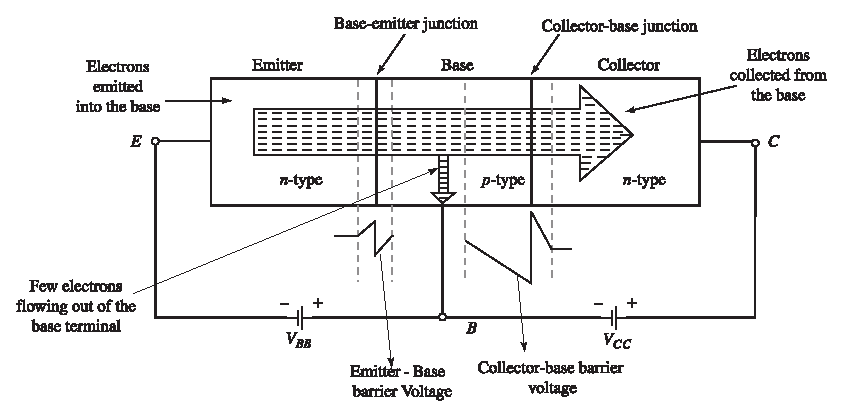
\includegraphics{chap2/S3-EE-03-004.eps}
\caption{$npn$ transistor in normal operation}\label{fig3.4}
\end{figure}

For normal operation, the emitter-base junction is forward-biased and the collector-base junction is reverse biased. The emitter-base junction is forward biased by applying negative voltage to the emitter with respect to the base. The collector-base junction is reverse biased by applying positive voltage to the collector with respect to the base.

The forward bias on emitter-base junction reduces the barrier voltage and causes the electrons to flow from the $n$-type emitter to the $p$-type base. The name emitter is due to the fact that electrons are emitted into the base region. Holes also flow from $p$-type base to the $n$-type emitter. Since the base is very lightly doped than the collector, almost all of the current flowing across the emitter-base junction is contributed by the electrons emitted from the emitter into the base. Thus, the majority charge carriers in $npn$ transistor are electrons.

The reverse bias at the collector-base junction causes the collector-base depletion region to penetrate deeper into the base than when the junction is unbiased. The electrons emitted from the emitter into the base arrive quite close to the large negative-positive electric filed at the collector-base depletion region. Since the electrons are negatively charged, they are drawn across the collector-base junction by this bias voltage. Thus the electrons emitted from emitter into the base are collected in the collector region. Hence the name collector.

The path from the emitter-base junction to the collector-base depletion region is much shorter than to the base terminal. So only a very small percentage of the total charge carriers entering the base from the emitter, flow out of the base terminal. Since the base region is very lightly doped, there are few holes in the base to recombine with electrons from the emitter, to form the base current. The recombination is only about 2\%. The remaining 98\% of charge carried from the emitter are drawn across the collector-base junction to flow through the collector terminal and the voltage sources back to the emitter.

\section[Operation of $pnp$ transistor]{Operation of \boldmath$pnp$ transistor}\label{sec3.4}
\index{pnp@$pnp$ transistor!operation of}

\vskip .1cm

Fig.~\ref{fig3.5} shows the depletion regions\index{pnp@$pnp$ transistor!depletion regions} and barrier voltages\index{pnp@$pnp$ transistor!barrier voltages} in an unbiased $pnp$ transistor.
%\begin{figure}[H]
%\centering
%\includegraphics{chap2/S3-EE-03-005.eps}
%\caption{Depletion region and barrier voltages in an unbiased $pnp$ transistor}\label{fig3.5}
%\end{figure}

\vskip .1cm

In an unbiased $pnp$ transistor, the barrier voltages are positive on the base and negative on the emitter and collector.

\vskip .1cm

As in the case of $npn$ transistor the emitter and collector layers are much more heavily doped than the base layer. As a result the depletion regions penetrate deep into the base, from either side.

\vskip .1cm

Fig.~\ref{fig3.6} shows a $pnp$ transistor with external bias voltages. For normal operation, the emitter-base junction is forward-biased and the collector-base junction is reverse biased. The emitter-base junction is forward biased by applying positive voltage to the emitter with respect to the base. The collector-base junction is reverse biased by applying negative voltage to the collector with respect to the base.

\vskip .1cm

The forward bias on emitter-base junction reduces the barrier voltage and causes the holes to flow from $p$-type emitter to the $n$-type base. Note that holes are emitted from the emitter in to the base. Electrons also flow from $n$-type base to the $p$-type emitter. Since the doping level of base is very small compared to that of collector, almost all of the current flowing across the emitter-base junction is contributed by the holes emitted from the emitter into the base. Thus, the majority charge carries in $pnp$ transistor are holes.
\begin{figure}[H]
\centering
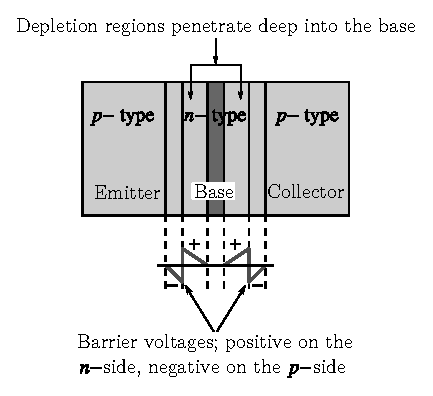
\includegraphics{chap2/fig2.5.eps}
\caption{Depletion region and barrier voltages in an unbiased $pnp$ transistor}\label{fig3.5}
\end{figure}

\begin{figure}[H]
\centering
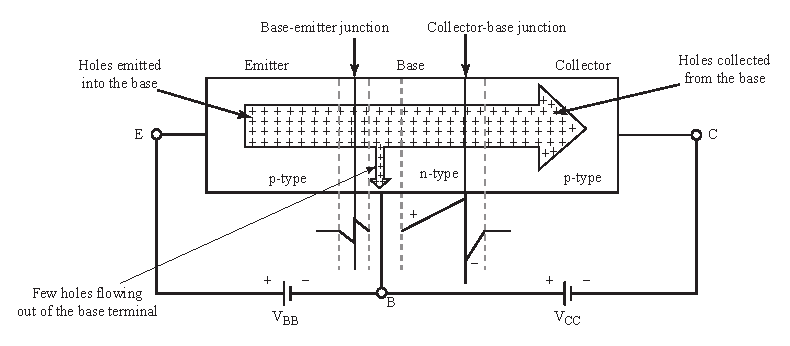
\includegraphics{chap2/S3-EE-03-006.eps}
\caption{$pnp$ transistor in normal operation}\label{fig3.6}
\end{figure}

The reverse bias at the collector-base junction causes the collector-base depletion region to penetrate deeper into the base than when the junction is unbiased. The holes emitted from the emitter into the base arrive quite close to the large positive-negative electric filed at the collector-base depletion region. Since the holes are positively charged, they are drawn across the collector-base junction by this bias voltage. Thus the holes emitted from emitter into the base are collected in the collector region.

The path from the emitter-base junction to the collector-base depletion region is much shorter than to the base terminal. So only a very small percentage of the total charge carriers entering the base from the emitter, flow out of the base terminal. Since the base region is very lightly doped, there are few electrons in the base to recombine with holes from the emitter, to form the base current. The recombination is only about 2\%. The remaining 98\% of charge carriers from the emitter are drawn across the collector-base junction to flow through the collector terminal and the voltage sources back to the emitter.

\section[Directions of $I_{E}$, $I_{C}$ and $I_{B}$ in $npn$ and $pnp$ transistors]{Directions of \boldmath$I_{E}$, $I_{C}$ and $I_{B}$ in $npn$ and $pnp$ transistors}\label{sec3.5}

Fig.~\ref{fig3.7} shows an $npn$ transistor for normal operation.
\begin{figure}[H]
\centering
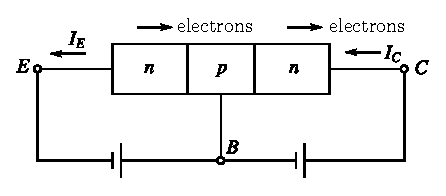
\includegraphics{chap2/fig2.7.eps}
\caption{$npn$ transistor biased for normal operation}\label{fig3.7}
\end{figure}

The forward bias on emitter-base junction pushes the electrons from $n$-emitter to the $p$-base. Note that electrons flow from $n$-emitter to the $p$-base. Hence the emitter current flows out of the emitter terminal, since the direction of current flow is opposite to the direction of electron flow.

At the collector, the electrons emitted from the emitter are collected. These collected electrons flow out of the collector terminal and enter the positive terminal of the supply, connected to the collector-base junction. As a result the collector current flows into the collector terminal.

Summing the transistor currents algebraically using KCL (taking incoming currents positive and out going currents negative), we have
\begin{align}
& -I_{E}+I_{B}+I_{C}=0\label{eq3.1}\\[3pt]
& I_{B}=I_{E}-I_{C}\label{eq3.2}
\end{align}

Since, $I_{E}>I_{C}$, $I_{B}$ is positive. Thus the direction of $I_{B}$ is into the base terminal.

Fig.~\ref{fig3.8} shows, the symbol of $npn$ transistor along with the directions of $I_{E}$, $I_{C}$ and $I_{B}$.

Performing the same analysis for $pnp$ transistor and using the fact that, the current flow is in the direction of holes flow, we can find the directions of $I_{E}$, $I_{C}$ and $I_{B}$. Fig.~\ref{fig3.9} shows, the symbol of $pnp$ transistor along with the directions of $I_{E}$, $I_{C}$ and $I_{B}$.
\begin{figure}[H]
\centering
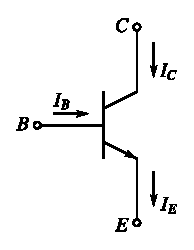
\includegraphics{chap2/fig2.8.eps}
\caption{$npn$ transistor with current directions\index{npn@$npn$ transistor!current directions}\index{pnp@$pnp$ transistor!current directions}}\label{fig3.8}
\end{figure}

\begin{figure}[H]
\centering
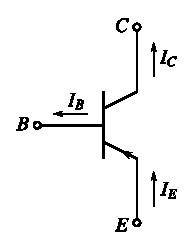
\includegraphics{chap2/fig2.9.eps}
\caption{$pnp$ transistor with current directions}\label{fig3.9}
\end{figure}

\noindent
{\bf Note:}~The directions of $I_{B}$ and $I_{C}$ are always opposite to the direction of $I_{E}$, in a BJT.

\section[Terminal voltages in an $npn$ transistor]{Terminal voltages in an \boldmath$npn$ transistor}\label{sec3.6}

Fig.~\ref{fig3.10}(a) shows the terminal voltages\index{npn@$npn$ transistor!terminal voltages} in an $npn$ transistor. The meaning of terminal voltages is as follows.
\begin{quote}
$V_{BE}$~: Base voltage with respect to emitter.

$V_{CB}$~: Collector voltage with respect to base.

$V_{CE}$~: Collector voltage with respect to emitter.
\end{quote}

In order to forward bias emitter-base junction in an $npn$ transistor, base voltage must be positive with respect to the emitter. Hence the polarity of $V_{BE}$ is shown positive at the base and negative at the emitter. The collector voltage must be negative with respect to the base, in order to reverse bias the collector-base junction. Hence the polarity of $V_{CB}$ is shown positive at the collector and negative at the base. Obviously, under this condition, the collector voltage will be positive with respect to emitter.
\begin{figure}[H]
\centering
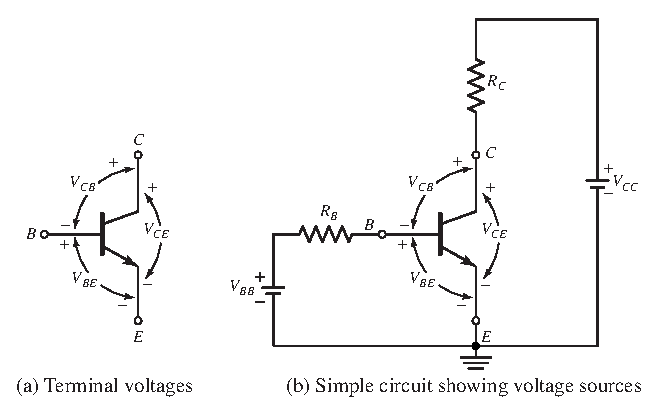
\includegraphics{chap2/S3-EE-03-007.eps}
\caption{Terminal voltages in an $npn$ transistor}\label{fig3.10}
\end{figure}

Fig.~\ref{fig3.10}(b) shows an $npn$ transistor biased by the dc sources $V_{BB}$ and $V_{CC}$. The base bias voltage, $V_{BB}$ is connected via resistor $R_{B}$ and the collector supply, $V_{CC}$ is connected via $R_{C}$. The negative terminals of $V_{BB}$ and $V_{CC}$ are connected at the transistor emitter terminal. To ensure reverse biasing of collector-base junction, $V_{CC}$ must be larger than $V_{BB}$. This keeps collector voltage positive with respect to base voltage.

Typical transistor voltages are as follows:
\begin{quote}
$V_{BE}$~: $0.7V$ for $S_{i}$ and $0.3V$ for $G_{e}$.

$V_{CE}$~: $3V$ to $20V$ for most of the transistors.
\end{quote}

\section[Terminal voltages in a $pnp$ transistor]{Terminal voltages in a \boldmath$pnp$ transistor}\label{sec3.7}

Fig.~\ref{fig3.11}(a) shows the terminal voltages\index{pnp@$pnp$ transistor!terminal voltages} in a $pnp$ transistor. The meaning of $V_{BE}$, $V_{CB}$ and $V_{CE}$ is same as that given for $npn$ transistor.

The polarity of $V_{BE}$ is shown positive at the emitter and negative at the base to indicate that emitter-base junction is forward biased. The reverse biasing on collector-base junction is indicated by the polarity of $V_{CB}$, which is positive at the base and negative at the collector.
\begin{figure}[H]
\centering
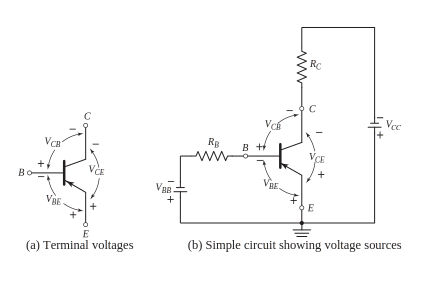
\includegraphics{chap2/S3-EE-03-008.eps}
\caption{Terminal voltages in a $pnp$ transistor}\label{fig3.11}
\end{figure}

Fig.~\ref{fig3.11}(b) shows a $pnp$ transistor biased by the dc sources $V_{BB}$ and $V_{CC}$. The base bias, $V_{BB}$ is connected via $R_{B}$ and the collector supply voltage, $V_{CC}$ is connected via $R_{C}$. The positive terminals of $V_{BB}$ and $V_{CC}$ are connected at the emitter terminal. To ensure reverse biasing of collector-base junction, $V_{CC}$ must be larger than $V_{BB}$. This keeps collector voltage negative with respect to base voltage.

\section{Transistor current gains}\label{sec3.8}
\index{Transistor!current gains}

The following two current gains are important in a BJT.
\begin{enumerate}
\item Emitter to collector current gain.

\item Base to collector current gain.
\end{enumerate}

\subsection{Emitter to collector current gain}\label{sec3.8.1}
\index{Current gain}

It is given by the ratio of dc collector current to dc emitter current. It is denoted by $\alpha_{\dc}$ and read as alpha dc.
\begin{equation}
\therefore\quad \alpha_{\dc}=\dfrac{I_{C}}{I_{E}}\label{eq3.3}
\end{equation}
$\alpha_{\dc}$ is also called the common base current gain.

Typically 96\% to 99.5\% of $I_{E}$ flows across the collector-base junction to form the collector current. Hence numerically $\alpha_{\dc}$ is typically 0.96 to 0.995.

\subsection{Base to collector current gain}\label{sec3.8.2}

It is given by the ratio of dc collector current to dc base current. It is denoted by $\beta_{\dc}$ and read as beta dc.
\begin{equation}
\therefore\quad \beta_{\dc}=\dfrac{I_{C}}{I_{B}}\label{eq3.4}
\end{equation}
$\beta_{\dc}$ is also called the common emitter current gain. Since $I_{C}\gg I_{B}$, $\beta_{\dc}\gg 1$.

Typically, $\beta_{\dc}$ ranges from 25 to 300.

$\beta_{\dc}$ is alternatively represented by $h_{FE}$, which originates from the $h$-parameter circuit of transistor. $h_{FE}$ is the symbol used an transistor data sheets.

\smallskip
\noindent
{\bf Note:}~The meaning of common base and common emitter will be explained in the later-sections.

\section[Reverse saturation current, $I_{CB0}$]{Reverse saturation current, \boldmath$I_{CB0}$}\label{sec3.9}
\index{Transistor!reverse saturation current}

Fig.~\ref{fig3.12} shows an $npn$ transistor with emitter-base junction open circuited and collector-base junction reverse biased.
\begin{figure}[H]
\centering
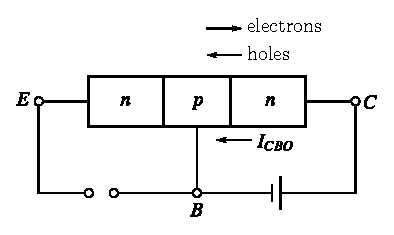
\includegraphics{chap2/fig2.12.eps}
\caption{$npn$ transistor with reverse bias on collector-base junction}\label{fig3.12}
\end{figure}

Reverse bias on collector-base junction results in minority carrier current flow across the junction.
\begin{itemize}
\item electrons flow from $p$-base to $n$-collector.

\item holes flow from $n$-collector to $p$-base.
\end{itemize}

As a result a reverse current flows from collector to base, even when the base emitter terminals are open. This current is called reverse saturation current,\index{Reverse saturation current} denoted by $I_{CB0}$ (collector to base reverse current with base emitter terminals open). This current is normally so small that it can be neglected. 

\section[To express $I_{C}$ in terms of $I_{B}$ and $\alpha_{\dc}$]{To express \boldmath$I_{C}$ in terms of $I_{B}$ and $\alpha_{\dc}$}\label{sec3.10}

We know that,
\begin{align}
I_{E} &=I_{C}+I_{B}\label{eq3.5}\\[5pt]
\text{Also,}\qquad \alpha_{\dc} &= \frac{I_{C}}{I_{E}}\notag\\[5pt]
\text{or},\qquad I_{C} &= \alpha_{\dc}I_{E}\label{eq3.6}
\end{align}
using Eqn.~\eqref{eq3.5} in \eqref{eq3.6}, we get
\begin{align}
I_{C} &= \alpha_{\dc}\,[I_{C}+I_{B}]\notag\\[5pt]
I_{C}\,[1-\alpha_{\dc}] &= \alpha_{\dc}\,I_{B}\notag\\[5pt]
\text{or},\qquad I_{C} &= \frac{\alpha_{\dc}}{1-\alpha_{\dc}}I_{B}\label{eq3.7}
\end{align}

\section[Relation between $\alpha_{\dc}$ and $\beta_{\dc}$]{Relation between \boldmath$\alpha_{\dc}$ and $\beta_{\dc}$}\label{sec3.11}

From Eqn.~\eqref{eq3.7}
$$
I_{C}=\frac{\alpha_{\dc}}{1-\alpha_{\dc}}I_{B}
$$
or
\begin{equation}
\frac{I_{C}}{I_{B}}=\dfrac{\alpha_{\dc}}{1-\alpha_{\dc}}\label{eq3.8}
\end{equation}

By definition,
\begin{equation}
\beta_{\dc}=\dfrac{I_{C}}{I_{B}}\label{eq3.9}
\end{equation}

From Eqns.~\eqref{eq3.8} and \eqref{eq3.9}
\begin{equation}
\beta_{\dc}=\dfrac{\alpha_{\dc}}{1-\alpha_{\dc}}\label{eq3.10}
\end{equation}

\eject

\section[$\beta_{\dc}$ in terms of $\alpha_{\dc}$]{\boldmath$\beta_{\dc}$ in terms of $\alpha_{\dc}$}\label{sec3.12}

From Eqn.~\eqref{eq3.10},
\begin{align}
\beta_{\dc} &= \frac{\alpha_{\dc}}{1-\alpha_{\dc}}\notag\\[4pt]
\text{or}\quad \beta_{\dc}(1-\alpha_{\dc}) &= \alpha_{\dc}\notag\\[4pt]
\beta_{\dc}-\beta_{\dc}\,\alpha_{\dc} &= \alpha_{\dc}\notag\\[4pt]
\beta_{\dc} &= \alpha_{\dc}+\beta_{\dc}\,\alpha_{\dc}\notag\\[4pt]
&= (1+\beta_{\dc})\alpha_{\dc}\notag\\[4pt]
\therefore\quad \alpha_{\dc} &= \frac{\beta_{\dc}}{1+\beta_{\dc}}\label{eq3.11}
\end{align}

\begin{example}\label{add3.1}
Show that
\begin{itemize}
\item[(a)] $I_{C}=\alpha_{\dc}I_{E}+I_{CE0}$ \ and

\item[(b)] $I_{C}=\beta I_{B}+(1+\beta)I_{CB0}$
\end{itemize}
\end{example}

\begin{solution}
\begin{itemize}
\item[(a)] Refer Fig.~\ref{fig3.12}.
\begin{itemize}
\item[$\bullet$] With base and emitter terminals open and collector-base junction reverse biased, the only current that flows through the collector-base junction is $I_{CB0}$.
\begin{equation*}
\therefore\qquad I_{C}=I_{CB0}\tag{A}
\end{equation*}

\item[$\bullet$] When the forward bias is also applied on the emitter-base junction, the collector current is
\begin{equation*}
I_{C}=\alpha_{\dc}I_{E}\tag{B}
\end{equation*}

\item[$\bullet$] The total collector current is given by
\begin{center}
\begin{tabular}{rp{5cm}cp{5cm}}
\raisebox{-.25cm}{$I_{C} \; = $} & Collector current due to forward bias on emitter-base junction & \raisebox{-.25cm}{+} & Collector current due to reverse bias on collector-base junction
\end{tabular}
\end{center}
\begin{equation*}
\therefore\qquad I_{C}=\alpha_{\dc}I_{E}+I_{CB0}\tag{C}
\end{equation*}
\end{itemize}

\item[(b)] $I_{E}=I_{B}+I_{C}$

Substituting this relation in Eqn.~(C), we have
\begin{align*}
I_{C} &=\alpha_{\dc}[I_{B}+I_{C}]+I_{CB0}\\[3pt]
I_{C} &= \alpha_{\dc}I_{B}+\alpha_{\dc}I_{C}+I_{CB0}\\[3pt]
I_{C}[1-\alpha_{\dc}] &= \alpha_{\dc}I_{B}+I_{CB0}\\[3pt]
I_{C} &= \dfrac{\alpha_{\dc}}{1-\alpha_{\dc}}I_{B}+\dfrac{1}{1-\alpha_{\dc}}I_{CB0}\tag{D}\\[3pt]
\text{But,}\qquad \beta_{\dc} &= \dfrac{\alpha_{\dc}}{1-\alpha_{\dc}}\tag{E}\\[3pt]
1+\beta_{\dc} &= \dfrac{\alpha_{\dc}}{1-\alpha_{\dc}}+1\\[3pt]
&= \dfrac{\alpha_{\dc}+1-\alpha_{\dc}}{1-\alpha_{\dc}}\\[3pt]
\therefore\quad 1+\beta_{\dc} &= \dfrac{1}{1-\alpha_{\dc}}\tag{F}
\end{align*}
Substituting Eqns.~(E) and (F) in Eqn.~(D), we get
\begin{equation*}
I_{C}=\beta_{\dc}I_{B}+[1+\beta_{\dc}]I_{CB0}\tag{G}
\end{equation*}
\end{itemize}
\vskip -.5cm
\end{solution}

\begin{example}\label{exam3.1}
Calculate the values of $I_{C}$, $I_{E}$ and $\beta_{\dc}$ for a transistor with $\alpha_{\dc}=0.98$ and \raisebox{4pt}{$I_{B}=120\,\mu A$.}
\end{example}

\begin{solution}
$$
I_{C}=\dfrac{\alpha_{\dc}}{1-\alpha_{\dc}}I_{B}
$$
Given, $\alpha_{\dc}=0.98$ and 
\begin{align*}
I_{B} = 120\, \mu A &= 0.12 \text{\,mA}\\[5pt]
I_{C} &= \frac{0.98}{1-0.98}(0.12\text{\,mA})\\[5pt]
\text{or}\qquad I_{C} &= 5.88\text{\,mA}\\[5pt]
I_{E} &= I_{C}+I_{B}\\[5pt]
&= (5.88\text{\,mA}+0.12\text{\,mA})\\[5pt]
&= 6\text{\,mA}\\[5pt]
\beta_{\dc} &= \frac{\alpha_{\dc}}{1-\alpha_{\dc}}=\frac{0.98}{1-0.98}=49\\[5pt]
\therefore\quad \beta_{\dc} &= 49
\end{align*}
\vskip -.75cm
\end{solution}

\begin{example}\label{exam3.2}
For the circuit shown in below, calculate
\begin{itemize}
\item[(a)] the values of $\alpha_{\dc}$ and $\beta_{\dc}$ of the transistor

\item[(b)] value of $I_{B}$ for a desired $I_{C}$ of $5{\rm\,mA}$.
\end{itemize}
\vskip -.5cm
\begin{figure}[H]
\centering
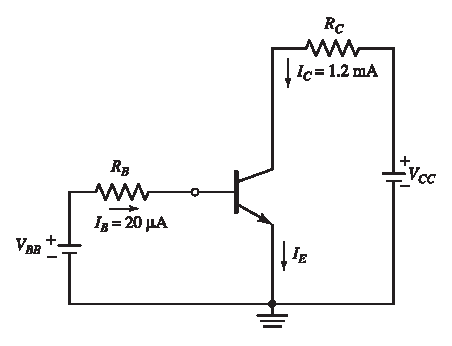
\includegraphics{chap2/S3-EE-03-011.eps}
\end{figure}
\end{example}

\begin{solution}
\begin{itemize}
\item[(a)]
~\phantom{a}
\vskip -.8cm
\begin{align*}
\beta_{\dc} &= \frac{I_{C}}{I_{B}}=\dfrac{1.2\text{\,mA}}{20\,\mu\text{A}}=\dfrac{1.2\,\text{mA}}{0.02\text{\,mA}}\\[3pt]
\text{or}\quad \beta_{\dc} &= 60\\[5pt]
\alpha_{\dc} &= \frac{\beta_{\dc}}{1+\beta_{\dc}}=\dfrac{60}{61}\\[3pt]
\text{or}\quad \alpha_{\dc} &= 0.984\\[5pt]
\alpha_{\dc} &= \frac{I_{C}}{I_{E}}\\[3pt]
\text{Now}\qquad I_{E} &= I_{C}+I_{B}\\[3pt]
&= 1.2\text{\,mA}+0.02\text{\,mA}=1.22\text{\,mA}
\end{align*}

\item[(b)] $I_{C}= 5\,\text{mA}$
\begin{align*}
I_{B} &= \dfrac{I_{C}}{\beta_{\dc}}= \dfrac{5\text{\,mA}}{60}\\[5pt]
      &= 83.33\,\mu\text{A}
\end{align*}
\end{itemize}
\vskip -.8cm
\end{solution}

\eject

\begin{example}\label{exam3.3}
Find $\alpha_{\dc}$, $I_{B}$ and $\beta_{\dc}$ for a transistor with $I_{C}=2.5\,\text{mA}$ and $I_{E}=2.55\,\text{mA}$.
\end{example}

\begin{solution}
\begin{align*}
\alpha_{\dc} &= \dfrac{I_{C}}{I_{E}}=\dfrac{2.5\text{\,mA}}{2.55\text{\,mA}}\\[5pt]
\text{or}\qquad\!\! \alpha_{\dc} &= 0.9804\\[7pt]
I_{E} &= I_{C}+I_{B}\\[6pt]
\text{or}\qquad I_{B} &= I_{E}-I_{C}=2.55\text{\,mA}-2.5\text{\,mA}=0.05\,\text{mA}\\[6pt]
\text{or}\qquad I_{B} &= 50\,\mu \text{A}\\[7pt]
\beta_{\dc} &= \dfrac{I_{C}}{I_{B}}=\dfrac{2.5\,\text{mA}}{0.05\text{\,mA}}\\[6pt]
\text{or}\qquad\!\!\! \beta_{\dc} &= 50
\end{align*}
Alternatively
$$
\beta_{\dc}=\dfrac{\alpha_{\dc}}{1-\alpha_{\dc}}=\dfrac{0.9804}{1-0.9804}=50.
$$
\vskip -.8cm
\end{solution}

\smallskip

\begin{example}\label{exam3.4}
A transistor circuit has $I_{C}=3\text{\,mA}$ and $I_{E}=3.03\text{\,mA}$. Find the $\beta_{\dc}$ of the transistor used. Assuming no change in the base current, find the new collector current when the transistor is replaced with a new one with $\beta_{\dc}$ of $70$.
\end{example}

\begin{solution}
The base current with the original transistor is
\begin{align*}
I_{B} &= I_{E}-I_{C}=(3.03\text{\,mA}-3.0\text{\,mA})=0.03\text{\,mA}\\[6pt]
\beta_{\dc} &= \frac{I_{C}}{I_{B}}=\dfrac{3\,\text{mA}}{0.03\,\text{mA}}=100
\end{align*}

\smallskip

The collector current with transistor of \ $\beta_{\dc}=70$ is
\begin{align*}
I_{C} &= \beta_{\dc}\,I_{B}\\[5pt]
&= 70\times 0.03\,\text{mA}\\[5pt]
\text{or}\qquad I_{C} &= 2.1\,\text{mA}
\end{align*}
\vskip -.8cm
\end{solution}

\eject

\begin{example}\label{exam3.5}
Find the values of $I_{C}$ and $I_{E}$ for a transistor with $\alpha_{\dc}=0.97$ and $I_{B}=50\,\mu \text{A}$. Find the $\beta_{\dc}$ of the transistor used.
\end{example}

\begin{solution}
$$
I_{C}=\dfrac{\alpha_{\dc}}{1-\alpha_{\dc}}I_{B}
$$
Now, $I_{B}=50\,\mu \text{A}=0.05\text{\,mA}$ and $\alpha_{\dc}=0.97$
\begin{align*}
\therefore\qquad I_{C} &= \frac{0.97}{1-0.97}(0.05\,\text{mA})\\[4pt]
\text{or}\qquad I_{C} &= 1.62\,\text{mA}
\end{align*}
By definition,
\begin{align*}
\alpha_{\dc} &= \dfrac{I_{C}}{I_{E}}\\[4pt]
\therefore\qquad I_{E} &= \dfrac{I_{C}}{\alpha_{\dc}}=\dfrac{1.62\,\text{mA}}{0.97}\\[4pt]
\text{or}\qquad I_{E} &= 1.67\text{\,mA}
\end{align*}
Again by definition,
\begin{align*}
\beta_{\dc} &= \frac{I_{C}}{I_{B}}=\dfrac{1.62\text{\,mA}}{0.05\text{\,mA}}\\[4pt]
\beta_{\dc} &= 32.4
\end{align*}
Alternatively,
$$
\beta_{\dc}=\dfrac{\alpha_{\dc}}{1-\alpha_{\dc}}=\dfrac{0.97}{1-0.97}=32.33
$$
\vskip -.7cm
\end{solution}

\smallskip

\begin{example}\label{exam3.6}
\begin{itemize}
\item[\rm(a)] Find $I_{E}$, $\alpha_{\dc}$ and $\beta_{\dc}$ of a transistor with $I_{C}=5.25\,\text{mA}$ and $I_{B}=100\,\mu\text{A}$

\item[\rm(b)] Find the new $I_{B}$ for an $I_{C}$ of $15\,\text{mA}$.
\end{itemize}
\end{example}

\begin{solution}
\begin{itemize}
\item[(a)] Given, $I_{C}=5.25\,\text{mA}$ and $I_{B}=100\,\mu \text{A}=0.1\,\text{mA}$
\begin{align*}
I_{E} &= I_{C}+I_{B}=(5.25\text{\,mA}+0.1\text{\,mA})\\[3pt]
\therefore\quad I_{E} &= 5.35\,\text{mA}
\end{align*}
By definition,
\begin{align*}
\alpha_{\dc} &= \dfrac{I_{C}}{I_{E}}=\dfrac{5.25\text{\,mA}}{5.35\text{\,mA}}=0.9813\\[3pt]
\beta_{\dc} &= \frac{I_{C}}{I_{B}}=\dfrac{5.25\text{\,mA}}{0.1\text{\,mA}}=52.5\\[3pt]
\text{or}\qquad \beta_{\dc} &= \dfrac{\alpha_{\dc}}{1-\alpha_{\dc}}=\dfrac{0.9813}{1-0.9813}=52.5
\end{align*}

\item[(b)] For a collector current of $I_{C}=15\,\text{mA}$,
\begin{align*}
I_{B} &= \dfrac{I_{C}}{\beta_{\dc}}=\dfrac{15\,\text{mA}}{52.5}=0.286\,\text{mA}\\[3pt]
\therefore\quad I_{B} &= 286\mu \text{A}
\end{align*}
\end{itemize}

Observe that for an increase in collector current from $5.25\,\text{mA}$ to $15\,\text{mA}$, the base current is required to be increased from $100\,\mu\text{A}$ to $286\,\mu\text{A}$.
\end{solution}

\begin{example}\label{exam3.7}
Find $I_{C}$ and $I_{E}$ for a transistor with $\alpha_{\dc}=0.99$ and $I_{B}=20\,\mu \text{A}$.
\end{example}

\begin{solution}
$$
I_{C}=\dfrac{\alpha_{\dc}}{1-\alpha_{\dc}}I_{B}
$$
Now, $I_{B}=20\,\mu\text{A}=0.02\text{\,mA}$ and $\alpha_{\dc}=0.99$
\begin{align*}
\therefore\quad I_{C} &= \frac{0.99}{1-0.99}(0.02\text{\,mA})\\[3pt]
\therefore\quad I_{C} &= 1.98\text{\,mA}\\[3pt]
I_{E} &= I_{C}+I_{B}\\[3pt]
&= (1.98\text{\,mA}+0.02\text{\,mA})\\[3pt]
\therefore\quad I_{E} &= 2\text{\,mA}
\end{align*}
\vskip -.8cm
\end{solution}

\begin{example}\label{exam3.8}
For a certain transistor circuit, $I_{C}=12.42\text{\,mA}$ and $I_{B}=200\,\mu\text{A}$.
\begin{itemize}
\item[\rm(a)] Find $I_{E}$

\item[\rm(b)] Find $\alpha_{\dc}$ and $\beta_{\dc}$ of the transistor

\item[\rm(c)] Find $I_{C}$ when $I_{B}=150\,\mu\text{A}$
\end{itemize}
\end{example}

\begin{solution}
Given, $I_{C}=12.42\text{\,mA}$ and $I_{B}=200\,\mu\text{A}=0.2\text{\,mA}$.
\begin{itemize}
\item[(a)] 
\begin{tabbing}
~~~~$I_{E}$ \== $I_{C}+I_{B}=(12.42\,\text{mA}+0.2\,\text{mA})$\\[6pt]
$\therefore$~ $I_{E}$ \>= $12.62\text{\,mA}$
\end{tabbing}

\medskip

\item[(b)]
\begin{tabbing}
\phantom{or\quad }$\alpha_{\dc}$ \== $\dfrac{I_{C}}{I_{E}}=\dfrac{12.42\text{mA}}{12.62\text{mA}}$\\[8pt]
\text{or}\quad $\alpha_{\dc}$ \>= $0.9842$\\[8pt]
\phantom{or\quad }$\beta_{\dc}$ \>= $\dfrac{I_{C}}{I_{B}}=\dfrac{12.42\text{mA}}{0.2\text{mA}}=62.1$
\end{tabbing}

\medskip

\item[(c)] When $I_{B}=150\,\mu\text{A}=0.15\text{\,mA}$,
\begin{align*}
I_{C} &= \beta_{\dc}\,I_{B}=(62.1)(0.15\text{\,mA})\\[5pt]
\therefore\qquad I_{C} &= 9.315\text{\,mA}
\end{align*}
\end{itemize}
\vskip -.8cm
\end{solution}

\medskip

\begin{example}\label{exam3.9}
A certain transistor circuit has $I_{C}=16\text{\,mA}$ and $I_{E}=16.04\text{\,mA}$. Find the new values of $I_{C}$ and $I_{E}$, for the same base current if the transistor is replaced with a transistor of $\beta_{\dc}=25$.
\end{example}

\begin{solution}
Given,
\begin{align*}
I_{C} &= 16\text{\,mA}\text{~~~ and~~~ }I_{E}=16.04\text{\,mA}\\[4pt]
I_{B} &= I_{E}-I_{C}=(16.04\text{\,mA}-16\text{\,mA})=0.04\text{\,mA}\\[4pt]
\therefore\qquad I_{B} &= 40\,\mu\text{A}
\end{align*}
For the existing transistor
$$
\beta_{\dc}=\dfrac{I_{C}}{I_{B}}=\dfrac{16\text{\,mA}}{0.04\text{\,mA}}=400
$$
When a transistor with $\beta_{\dc}=25$ is used,
\begin{align*}
I_{C} &= \beta_{\dc}\,I_{B}=25\times 0.04\text{\,mA}\\[4pt]
\therefore\qquad I_{C} &= 1\text{\,mA}\\[4pt]
\text{and}\qquad I_{E} &= I_{C}+I_{B}=(1\text{\,mA}+0.04\text{\,mA})\\[4pt]
\therefore\qquad I_{E} &= 1.04\text{\,mA}
\end{align*}
\vskip -.8cm
\end{solution}

\eject

\section{Transistor configurations}\label{sec3.13}
\index{Transistor configurations}\index{Transistor!transistor configurations}

Almost all electronic circuits are represented by a two port, four terminal network as shown in Fig.~\ref{fig3.13}.
\begin{figure}[H]
\centering
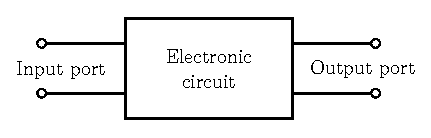
\includegraphics{chap2/fig2.13.eps}
\caption{Two port representation of an electronic circuit}\label{fig3.13}
\end{figure}

Since BJT has only three terminals, one of the three terminals is made common for both input and output ports, in order to use it as a two port device. This leads to the following three configurations of BJT.
\begin{enumerate}
\item Common-emitter (CE) configuration

\item Common-base (CB) configuration

\item Common-collector (CC) configuration
\end{enumerate}

\subsection{Common-emitter configuration}\label{sec3.13.1}

In common-emitter configuration,\index{Common-emitter configuration}\index{Transistor configurations!ce configuration} the emitter terminal is made common between input and output ports as shown in Fig.~\ref{fig3.14}.
\begin{figure}[H]
\centering
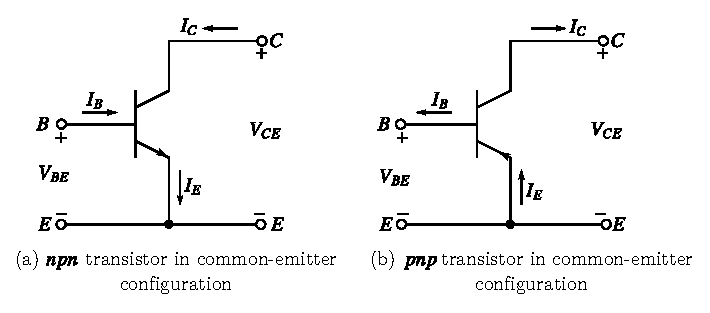
\includegraphics{chap2/fig2.14.eps}
\caption{Common-emitter configuration}\label{fig3.14}
\end{figure}

\eject

The following observations are made from Fig.~\ref{fig3.14}.
\begin{quote}
input current~:~ $I_{B}$

output current~:~ $I_{C}$

input voltage~:~ $V_{BE}$

output voltage~:~ $V_{CE}$
\end{quote}

\subsection{Common-base configuration}\label{sec3.13.2}

In common-base configuration,\index{Common-base configuration}\index{Transistor configurations!cb configuration} the base terminal is made common between input and output ports as shown in Fig.~\ref{fig3.15}.
\begin{figure}[H]
\centering
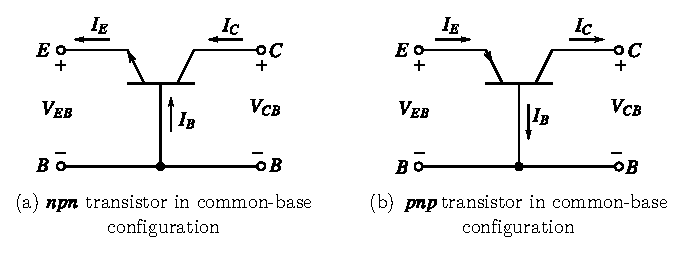
\includegraphics{chap2/fig2.15.eps}
\caption{Common-base configuration}\label{fig3.15}
\end{figure}

We note the following from Fig.~\ref{fig3.15}.
\begin{quote}
input current~:~ $I_{E}$

output current~:~ $I_{C}$

input voltage~:~ $V_{EB}$

output voltage~:~ $V_{CB}$
\end{quote}

\subsection{Common-collector configuration}\label{sec3.13.3}

In common-collector configuration,\index{Common-collector configuration}\index{Transistor configurations!cc configuratoin} the collector terminal is made common between input and output ports as shown in Fig.~\ref{fig3.16}.

From Fig.~\ref{fig3.16}, we note the following,
\begin{quote}
input current~:~ $I_{B}$

output current~:~ $I_{E}$

input voltage~:~ $V_{BC}$

output voltage~:~ $V_{EC}$
\end{quote}
\begin{figure}[H]
\centering
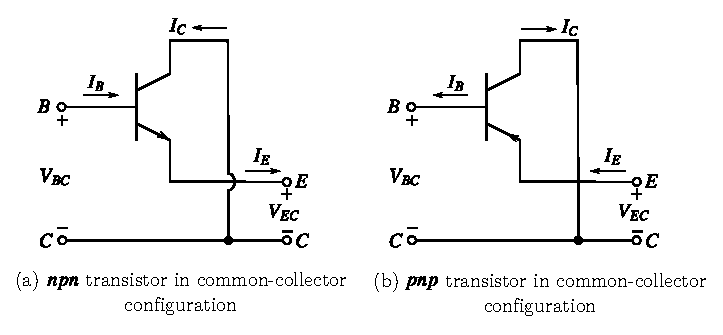
\includegraphics[scale=.95]{chap2/fig2.16.eps}
\caption{Common-collector configuration}\label{fig3.16}
\end{figure}

\section{BJT current amplification}\label{sec3.14}

Current amplification or current gain\index{Current gain} is given by the ratio of output current to the input current. In common-emitter configuration the output current, $I_{C}$, is very much larger than the input current, $I_{B}$. Hence, common-emitter configuration is capable of amplifying the current.

The current gain can be measured under two conditions
\begin{enumerate}
\itemsep=0pt
\item When the currents are constant, which gives dc current gain.

\item When the currents are changing, which gives ac current gain.
\end{enumerate}

The common-emitter dc current gain, $\beta_{\dc}$ was discussed in Section \ref{sec3.8.2}.

\subsection[Common-emitter ac current gain $(\,\beta_{\ac}\,)$]{Common-emitter ac current gain \boldmath$(\,\beta_{\ac}\,)$}\label{sec3.14.1}
\index{Current gain!ce}

When the base current increases by $\Delta I_{B}$, the collector increases by $\Delta I_{C}$ and the emitter current by $\Delta I_{E}$. Similarly, when the base current decreases by $\Delta I_{B}$, the collector current decreases by $\Delta I_{C}$ and the emitter current by $\Delta I_{E}$. The common-emitter ac current is given by the ratio of change in collector current to change in base current, denoted by $\beta_{\ac}$.
\begin{equation}
\beta_{\ac}=\dfrac{\Delta I_{C}}{\Delta I_{B}}\label{eq3.12}
\end{equation}

The increasing and decreasing levels of input and output currents may be defined as alternating quantities. AC quantities are represented by upper case letter with lower case subscript.
\begin{align*}
\therefore\qquad & I_{b}\text{~ is ac base current}\\
                 & I_{c} \text{~ is ac collector current}
\end{align*}
Thus, $\beta_{\ac}$ is ac current gain from base to collector.

\vfill\eject

Hence,
\begin{equation}
\beta_{\ac}=\frac{I_{c}}{I_{b}}\label{eq3.13}
\end{equation}
$\beta_{\ac}$ is also called the common-emitter ac current gain. On transistor data sheets, $\beta_{\ac}$ is alternatively represented by $h_{fe}$.

A small change in the base current, produces a large change in collector current. Hence, $\beta_{\ac}\gg 1$. For a transistor, $\beta_{\dc}$ and $\beta_{\ac}$ have almost, same range of values.

Thus,
\begin{equation}
\beta_{\ac}\approx \beta_{\dc}\label{eq3.14}
\end{equation}

\section{Voltage amplification in BJT}\label{sec3.15}

Fig.~\ref{fig3.17} shows an $npn$ transistor biased for normal operation.
\begin{figure}[H]
\centering
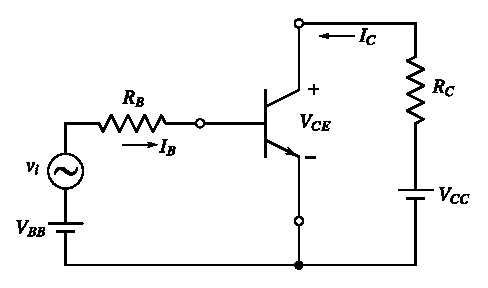
\includegraphics{chap2/fig2.17.eps}
\caption{$npn$ transistor biased for normal operation}\label{fig3.17}
\end{figure}
\noindent
$v_{i}$ is the ac voltage (ac signal) to be amplified. It is connected in the base-emitter circuit. We intend to take the ac output between collector and emitter terminals. Hence the configuration is common-emitter.

Let the ac input voltage change by an amount, $\Delta V_{B}$. The consequences are as follows
\begin{itemize}
\item The base current changes by $\Delta I_{B}$

\item Collector current changes by
\begin{equation}
\Delta I_{C}=\beta_{\dc}\,\Delta I_{B}\label{eq3.15}
\end{equation}
\end{itemize}
Let us find the change in output voltage, $V_{CE}$.

Applying KVL to collector-emitter circuit, we have \ $V_{CC}-I_{C}R_{C}-V_{CE}=0$.
\begin{equation}
V_{CE}=V_{CC}-I_{C}R_{C}\label{eq3.16}
\end{equation}

Change in output voltage, $\Delta V_{CE}$, is given by
\begin{equation}
\Delta V_{CE}=-\,\Delta I_{C}\,R_{C}\label{eq3.17}
\end{equation}
[Since $V_{CC}$ is constant, $\Delta V_{CC}=0$]

\vskip .1cm
Using Eqn.~\eqref{eq3.15} in \eqref{eq3.17} we have
\begin{equation}
\Delta V_{CE}=-\beta_{\dc}\,\Delta I_{B}\,R_{C}\label{eq3.18}
\end{equation}

Voltage amplification or voltage gain\index{Voltage gain}\index{Transistor!voltage gain}\index{Common-emitter configuration!voltage gain} is given by the ratio of change in output voltage to the change in input voltage, denoted by, $A_{V}$.
\begin{align}
\therefore\qquad A_{V} &= \dfrac{\Delta V_{CE}}{\Delta V_{B}}\label{eq3.19}\\[5pt]
\text{or}\qquad A_{V} &= \frac{-\beta_{\dc}\,\Delta I_{B}\,R_{C}}{\Delta V_{B}}\label{eq3.20}
\end{align}

To get an estimate of $A_{V}$, we assume the following values for circuit components and transistor parameters.
\begin{align*}
\text{Let},\qquad R_{C} &= 12\, k\Omega\quad\text{and}\quad \beta_{\dc}=50
\end{align*}
Also let the change, $\Delta V_{B}=\pm\, 20\,\text{mV}$ results in $\Delta I_{B}=\pm\, 5\,\text{mA}$.

Using these values in Eqn.~\eqref{eq3.20}, we have
\begin{align*}
A_{V} &= \frac{-(50)(\pm 5\text{mA})(12 k\Omega)}{(\pm 20\text{mV})}=-150\\[3pt]
\text{or}\qquad |\,A_{V}\,| &= 150
\end{align*}
From Eqn.~\eqref{eq3.19} we have
$$
\Delta V_{CE}=A_{V}\,\Delta V_{B}\quad\text{or}\quad \Delta V_{CE}=-150\Delta V_{B}
$$
or \ change in output voltage = $-150$ times the change in input voltage.

\vskip .1cm

Hence, common-emitter configuration is capable of amplifying the voltage. The negative sign in $A_{V}$ implies that, in common-emitter configuration the input and output voltages are $180^{\circ}$ out of phase.

\eject

\begin{example}\label{exam3.10}
The amplifier shown in Fig.~(A) has transistor with $\beta_{\dc}=\beta_{\ac}=80$ and has the input characteristic shown in Fig.~(B). Find:

\vskip .1cm

(a) the $\dc$ collector voltage\quad (b) voltage gain of the circuit for a $v_{i}$ of $\pm 50$\,mV.
\begin{figure}[H]
\centering
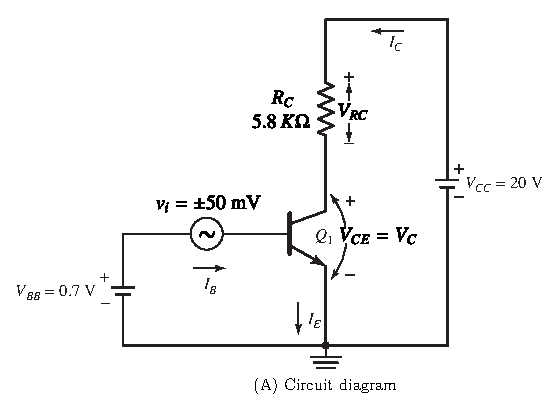
\includegraphics[scale=1.1]{chap2/S3-EE-03-014a.eps}
\end{figure}
\begin{figure}[H]
\centering
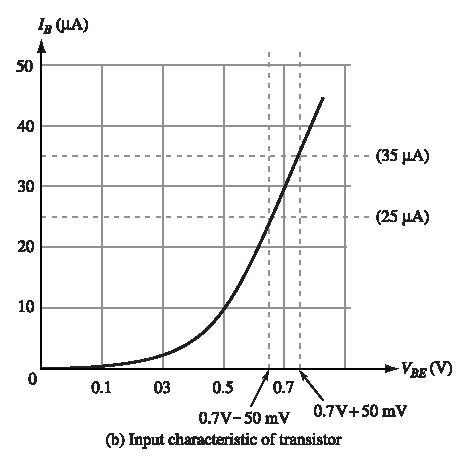
\includegraphics[scale=1.1]{chap2/S3-EE-03-014b.eps}
\end{figure}
\end{example}

\eject

\begin{solution}
From the characteristics, $I_{B}=30\,\mu\text{A}$~ for~ $V_{BE}=0.7\text{V}$.

By definition,
\begin{align*}
\beta_{\dc} &= \frac{I_{C}}{I_{B}}\\[4pt]
\therefore\quad I_{C} &= \beta_{\dc}\,I_{B}=80\times (30\,\mu\text{A})=80\times (0.03\,\text{mA})\\[4pt]
\therefore\quad I_{C} &= 2.4\,\text{mA}
\end{align*}
Now, writing Kirchhoff's Voltage Law equation for the collector-emitter circuit, we get
\begin{align*}
V_{CC} &= V_{RC}+V_{CE}\Rightarrow V_{CE}=V_{CC}-I_{C}R_{C}\\[5pt]
\text{where}\quad V_{R_{C}} &= \text{voltage across resistor $R_{C}$}\\[5pt]
 &= I_{C}\,R_{C}\\[5pt]
\therefore\quad V_{CE} &= 20-(2.4\text{\,mA}\times 5.8 k\Omega)\\[5pt]
\therefore\quad V_{CE} &= 6.08\text{\,V}=V_{C}
\end{align*}

From the input characteristic shown, for $\Delta v_{i}$ \ or \ $\Delta V_{B}=\pm 50\,\text{mV}$,
\begin{align*}
\Delta I_{B} &= \pm 5\,\mu\text{A}\\[5pt]
\text{or}\quad I_{b} &= \pm 5\,\mu\text{A}\\[5pt]
\therefore\qquad I_{c}&=\beta_{\ac}\,I_{b}\\[5pt]
&= 80\times (\pm 5\,\mu\text{A})=\pm 400\,\mu \text{A}\\[5pt]
I_{c} &= \pm 0.4\text{\,mA}
\end{align*}
we have
\begin{align*}
V_{CE} &= V_{CC}-I_{C}\,R_{C}\\[4pt]
\Delta V_{CE} &= \Delta V_{CC}-\Delta I_{C}\,R_{C}\\[4pt]
\text{or}\qquad V_{ce} &= -I_{c}\,R_{C}\quad[\because \ \Delta V_{CC}=0]\\[4pt]
\text{or}\qquad V_{0} &= - (\pm 0.4\text{mA})(5.8k\Omega)\\[4pt]
V_{0} &= \mp\, 2.32\text{V}
\end{align*}
\indent
Therefore, voltage gain
\begin{align*}
A_{V} &= \frac{V_{o}}{V_{i}}=\frac{\mp\, 2.32\text{V}}{\pm 50\,\text{mV}}\\[3pt]
\therefore\qquad A_{V} &= -46.4\quad\text{or}\quad |\,A_{V}\,|=46.4
\end{align*}
\vskip -.8cm
\end{solution}

\eject

\begin{example}\label{exam3.11}
\begin{itemize}
\item[(a)] Find the $\dc$ current gain for the circuit shown below.

\item[(b)] Find the $\ac$ voltage gain for an input of $\pm 50\text{\,mV}$. Assume that a $\pm 50\,\text{mV}$ input voltage change corresponds to a $\pm 10\,\mu\text{A}$ change in the base current.
\begin{figure}[H]
\centering
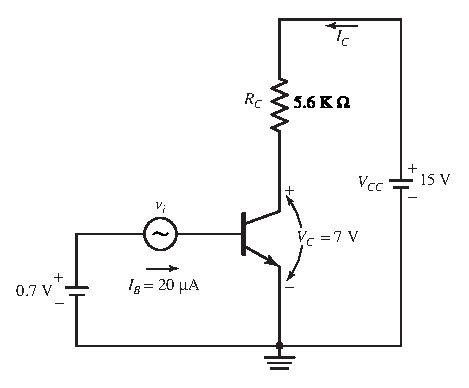
\includegraphics{chap2/S3-EE-03-015.eps}
\end{figure}
\end{itemize}
\end{example}

\begin{solution}
\begin{itemize}
\item[(a)] From the Figure given,
\begin{align*}
V_{R_{C}} &= V_{CC}-V_{C}\\[2pt]
&= 15\V-7\V=8\text{\,V}\\[2pt]
V_{R_{C}} &= 8\text{\,V}\\[2pt]
\text{or}\qquad I_{C}\,R_{C} &= 8\text{\,V}\\[2pt]
\therefore\quad I_{C} &= \dfrac{8\text{V}}{5.6k\Omega}\\[2pt]
\text{or}\qquad I_{C} &= 1.43\text{\,mA}\\[2pt]
\text{By definition~~ } \beta_{\dc} &=\dfrac{I_{C}}{I_{B}}=\dfrac{1.43\text{mA}}{0.02\text{mA}}\\[2pt]
\text{or}\qquad \beta_{\dc} &= 71.5
\end{align*}

\item[(b)] Given that for $\Delta V_{B}=\pm 50\text{\,mV}$, $\Delta I_{B}=\pm 10\mu\text{A}$
\begin{align*}
\Delta I_{C} &= \beta_{\dc}\,\Delta I_{B}\\[2pt]
&= (71.5)(\pm 10\mu\text{A})\\[2pt]
\therefore\qquad \Delta I_{C} &= I_{c}=\pm 0.715\text{\,mA}\\[2pt]
\text{and}\qquad V_{o} &= -I_{c}R_{C}=-(\pm\, 0.715\text{\,mA})(5.6 k\Omega)\\[2pt]
\therefore\qquad V_{o} &= \mp\, 4\,\text{V}\\[2pt]
\therefore\qquad A_{V} &= \frac{V_{o}}{V_{1}}=\dfrac{\mp\,4\text{V}}{\mp\,50\text{\,mV}}=\dfrac{\mp\,4\text{V}}{\mp\,0.05\text{V}}\\[2pt]
\therefore\qquad A_{V} &= -80\quad\text{or}\quad |\,A_{V}\,|=80
\end{align*}
\end{itemize}
\vskip -.5cm
\end{solution}

\begin{example}\label{exam3.12}
The circuit shown in Fig.~(A) uses a transistor with $\beta_{\dc}=50$ and with input characteristics as shown in Fig.~(B).
\begin{figure}[H]
\centering
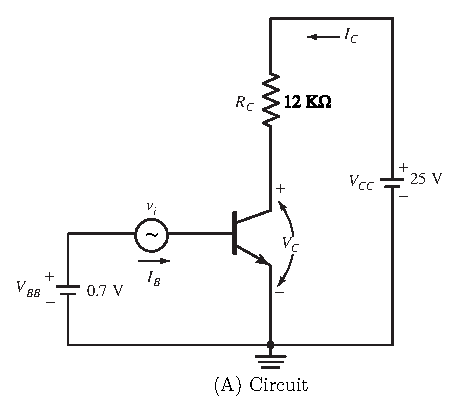
\includegraphics{chap2/S3-EE-03-016a.eps}

\smallskip
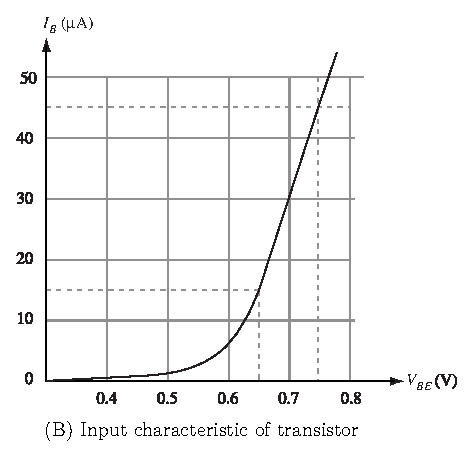
\includegraphics{chap2/S3-EE-03-016b.eps}
\end{figure}
\begin{itemize}
\item[(a)] Find collector voltage.

\item[(b)] Find voltage gain for $v_{i}=\pm 50\text{\,mV}$.

\item[(c)] Find $V_{CE}$ if $V_{BE}=0.73\text{V}$ instead of $0.7\text{V}$.

\item[(d)] Find voltage gain when $R_{C}$ is changed to $6.8\, k\Omega$.

\item[(e)] When the transistor is replaced in the circuit in Fig.~(A) and $V_{C}=9\text{V}$, assuming $I_{B}$ remains the same, find the current gain of the replaced transistor.
\end{itemize}
\end{example}

\begin{solution}
\begin{itemize}
\item[(a)] From Fig.~(A) for $V_{BE}=0.7\text{V}$, $I_{B}=30\mu \text{A}$
\begin{align*}
\therefore\qquad I_{C}&=\beta_{\dc}I_{B}=50\times 0.03\text{\,mA}\\[4pt]
\text{or}\qquad I_{C} &= 1.5\text{\,mA}\\[4pt]
V_{C} &= V_{CC}-I_{C}R_{C}\\[4pt]
&= 25V-(1.5\text{mA})(12k\Omega)\\[4pt]
\text{or}\qquad V_{C} &= 7\text{V}
\end{align*}

\item[(b)] From Fig.~(B) for a variation of $v_{i}$ or $V_{BE}$ of $\pm 50\text{\,mV}$, variation in $I_{B}$ is $\pm 15\,\mu\text{A}$.
\begin{align*}
\therefore\qquad \Delta I_{B} &= \pm 15\,\mu\text{A}\\[4pt]
\therefore\qquad \Delta I_{C} &= \beta_{\dc}\,I_{B}\\[4pt]
&= 50\times (\pm 15\,\mu\text{A})\\[4pt]
\Delta I_{C} &= \pm 0.75\text{~mA}=I_{c}\\[4pt]
\therefore\qquad V_{o} &= -I_{c}R_{C}=-(\pm 0.75\text{\,mA})(12 k\Omega)\\[4pt]
\therefore\qquad &= \mp\, 9\text{V}\\[4pt]
\therefore\qquad A_{V} &= \frac{V_{o}}{V_{1}}=\dfrac{\mp\,9\text{V}}{\pm\,50\text{\,mV}}=\frac{\mp\,9\text{V}}{\pm\,0.05\text{V}}\\[4pt]
\therefore\qquad A_{V} &= -180\quad\text{or}\quad |A_{V}|=180
\end{align*}

\eject

\item[(c)] From Fig.~(B) when $V_{BE}=0.73\text{V}$, $I_{B}=40\,\mu\text{A}$
\begin{align*}
\therefore\qquad I_{C} &= \beta_{\dc}\,I_{B}=50\times (0.04\text{\,mA})\\[4pt]
\text{or}\qquad I_{C} &= 2\text{\,mA}\\[4pt]
\therefore\qquad V_{CE} &= V_{C}=V_{CC}-V_{R_{C}}\\[4pt]
&= V_{CC}-I_{C}R_{C}\\[4pt]
&= 25-(2\text{\,mA})(12 k\Omega)\\[4pt]
V_{CE} &= 1\text{V}
\end{align*}

\item[(d)] From part (b),
\begin{align*}
I_{c} &= \pm 0.75\text{mA}\\[3pt]
V_{0} &= -I_{c}\,R_{C}\\[3pt]
&= -(\pm 0.75\text{\,mA})(6.8k\Omega)\\[3pt]
&= \mp\, 5.1\text{V}\\[3pt]
\therefore\qquad A_{V} &= \frac{V_{0}}{V_{1}}=\frac{\mp\,5.1\text{V}}{\pm\,0.05\text{V}}=-102\quad\text{or}\quad |A_{V}|=102
\end{align*}
Observe that decrease in $R_{C}$ reduces the voltage gain

\item[(e)] With the changed transistor, $V_{C}=9\text{V}$.

Therefore from Fig.~(A)
\begin{align*}
V_{R_{C}} &= V_{CC}-V_{C}=25V-9V=16\text{V}\\[4pt]
\therefore\qquad I_{C}\,R_{C} &= 16\text{V}\\[4pt]
\text{or}\qquad I_{C} &= \dfrac{16\text{V}}{12 k\Omega}=1.33\text{\,mA}\\[4pt]
\therefore\qquad \beta_{\dc} &= \frac{I_{C}}{I_{B}}=\dfrac{1.33\text{mA}}{30\mu\text{A}}=\frac{1.33\text{mA}}{0.03\text{mA}}\\[4pt]
\therefore\qquad \beta_{\dc} &= 44.33
\end{align*}
\end{itemize}
\vskip -.8cm
\end{solution}

\eject

\section{Transistor characteristics}\label{sec3.16}
\index{Transistor characteristics}

Following are the characteristics\index{Transistor!characteristics} that can be investigated for a transistor.
\begin{enumerate}
\item Input characteristics

\item Output characteristics

\item Current gain characteristics
\end{enumerate}
\begin{itemize}
\item[$\bullet$]
Input characteristics of a transistor is studied by plotting input current as a function of input voltage, keeping the output voltage constant.

\item[$\bullet$]
Output characteristics of a transistor is investigated by plotting output current as a function of output voltage, keeping the input current constant.

\item[$\bullet$]
The current gain characteristics of a transistor is obtained by plotting output current as a function of input current, keeping the output voltage constant.
\end{itemize}
Now let us study these characteristics for all the three configurations of the transistor.

\section{Common-Base input characteristics}\label{sec3.17}

The input characteristics\index{Common-base configuration!input characteristics} of common-base configuration\index{Transistor characteristics!cb configuration} is obtained by plotting, the input current, $I_{E}$, as a function of input voltage, $V_{EB}$, keeping the output voltage, $V_{CB}$, constant.

\vskip .1cm
The circuit for investigating BJT common-base characteristics is shown in Fig.~\ref{fig3.18}.

For $pnp$ transistor, $V_{EB}$ is positive for forward bias on emitter-base junction and $V_{CB}$ is negative for reverse bias on collector-base junction.
\begin{figure}[H]
\centering
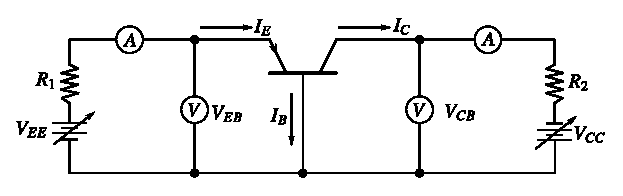
\includegraphics{chap2/fig2.18.eps}
\caption{Circuit for investigating BJT common-base characteristics}\label{fig3.18}
\end{figure}

The output voltage $V_{CB}$, is kept constant and the input voltage, $V_{EB}$ is set at several convenient levels. At each level of $V_{EB}$, the corresponding input current, $I_{E}$ is recorded. When this procedure is repeated for different $V_{CB}$ levels, a family of input characteristic curves are obtained as shown in Fig.~\ref{fig3.19}.
\begin{figure}[H]
\centering
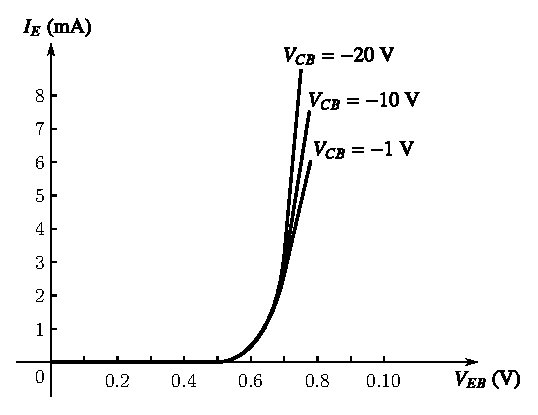
\includegraphics{chap2/fig2.19.eps}
\caption{Input characteristic of common-base configuration}\label{fig3.19}
\end{figure}

The following observations are made from the input characteristics of Fig.~\ref{fig3.19}.
\begin{itemize}
\itemsep=2pt
\item The characteristics are essentially those of a forward-biased $p$-$n$ junction, since the emitter-base junction under forward bias is similar to a forward biased $p$-$n$ junction.

\item At a given input voltage, $V_{EB}$, the input current, $I_{E}$, increases with increase in $V_{CB}$. This is indicated by the shift of input characteristic curves to the left with increase in $V_{CB}$. This can be accounted as follows. At larger $V_{CB}$ (larger reverse bias voltage), the depletion region at the collector-base junction penetrates deeper into the base of transistor, thus shortening the distance. This reduces the resistance the emitter-base and collector-base junctions. As a result, the input current, $I_{E}$, increases.

\item A small change in $V_{EB}$ causes a large change in $I_{E}$. This means that the dynamic input impedance of common-base configuration is low.
\end{itemize}

\eject

\section{Common-Base output characteristics}\label{sec3.18}

The circuit shown in Fig.~\ref{fig3.18} can also be used to investigate the output characteristics.\index{Common-base configuration!output characteristics}

\vskip .1cm

For plotting the output characteristics, the input current, $I_{E}$, is held constant and the output voltage, $V_{CB}$, is adjusted in convenient steps, and the corresponding values of output current, $I_{C}$, are recorded. If the procedure is repeated for different $I_{E}$ settings, we get a family of output characteristics as shown in Fig.~\ref{fig3.24}.
\begin{figure}[H]
\centering
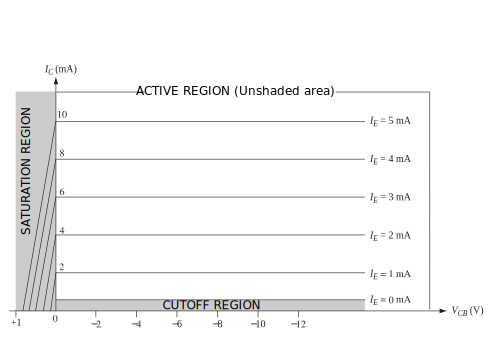
\includegraphics{chap2/S3-EE-03-019.eps}
\caption{Output characteristics of common-base configuration}\label{fig3.24}
\end{figure}

The following observations are made from the output characteristics shown in Fig.~\ref{fig3.24}.
\begin{itemize}
\item Since $I_{E}$ is fixed and $I_{C}\approx I_{E}$, the collector current varies very little, when $V_{CB}$ is increased. Thus the characteristic curves are almost parallel to $V_{CB}$ axis.

\item This is due to the fact that, with an increase in $V_{CB}$, the collector-base depletion region, widens shortening the distance between the two depletion regions. Hence a large increase in $V_{CB}$ is required to bring about a small change in $I_{C}$, with $I_{E}$ held constant. Thus the output characteristic curves are almost parallel to $V_{CB}$ axis. This is called Early effect.

\item Since the output current $I_{C}$ is almost equal to the input current $I_{E}$, the current gain is unity in common-base configuration.

\item Since $I_{C}$ varies very little with $V_{CB}$ the output resistance $\dfrac{\Delta V_{CB}}{\Delta I_{C}}$ is very high in common-base configuration.

\item The collector current flows even when $V_{CB}$ is zero. This is because, there is still a barrier voltage at the collector-base junction, which assists the flow of $I_{C}$, even when $V_{CB}=0$.

\item The following regions of operation are identified on the output characteristics. 
\end{itemize}

\smallskip
\heading{(a) Saturation region}

The collector current is reduced to zero only when $V_{CB}$ is increased positively. Positive $V_{CB}$ for $pnp$ transistor implies forward bias on collector-base junction and the transistor is said to operate in saturation region. The region on the graph to the left of $I_{C}$ axis is called saturation region. 

{\em In saturation region emitter-base junction and collector-base junction are both forward biased.}

\smallskip
\heading{(b) Active region}


The region which lies to the right of $I_{C}$ axis and above the characteristic curve corresponding to $I_{E}=0$, is called the active region. This is the normal operating region for the transistor.

{\em In the Active region emitter-base junction is forward biased and collector-base junction is reverse biased.}

\smallskip
\heading{(c) Cut-off region}


The region to the right of $I_{C}$ axis and below the characteristic curve corresponding to $I_{E}=0$ (very close to $V_{CB}$ axis), is called the cut-off region.

\vskip .1cm

{\em In cut-off region both emitter-base and collector-base junctions are reverse biased.}

\vskip .1cm

If an excessive reverse-bias voltage, $V_{CB}$ is applied to the collector-base junction, the device breakdown may occur.\\[-20pt]

\subsection{Suitability of operating regions for the intended application of transistor}\label{sec3.18.1}

When ever the transistor is to be used as an amplifier, it must be biased in the active region i.e., emitter-base junction forward biased and collector-base junction reverse biased. It is the linear region of operation for the transistor and it can faithfully amplify the input signal with minimum distortion. 

\vskip .15cm

When the transistor is to be used as a switch, it must be operated between cut-off and saturation.

\subsection{Breakdown in transistor}\label{sec3.18.2}

The transistor may breakdown,\index{Transistor!breakdown} when an excessive reverse-bias voltage is applied to the collector-base junction. Breakdown is caused by the following two effects.
\begin{itemize}
\item The collector-base junction breaks down due to the flow of large reverse saturation current through the junction. This is similar to reverse breakdown of junction in a $pn$ diode. 

\item When the reverse bias voltage, $V_{CB}$, exceeds the maximum value specified by the manufacturer, the collector-base depletion region may penetrate deep into the base until it comes into contact with emitter-base depletion region. This condition is called punch-through\index{Transistor!punch-through} or reach-through and is shown in Fig.~\ref{fig3.25}.
\end{itemize}

The collector-base depletion region extending upto the emitter-base depletion region causes punch-through leading to the flow of excessive current through the device resulting in its damage.

\vskip .1cm

Typical maximum values of $V_{CB}$ range between 25V and 80V for low voltage devices.
\begin{figure}[H]
\centering
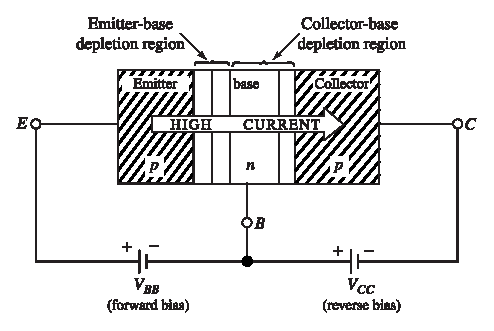
\includegraphics[scale=1.15]{chap2/S3-EE-03-024.eps}
\caption{Illustration of punch-through\index{Punch-through}}\label{fig3.25}
\end{figure}

\section{Current gain characteristics of common-base configuration}\label{sec3.19}
\index{Common-base configuration!current gain characteristics}

The current gain characteristics\index{Current gain characteristics} is also called the forward transfer characteristics.\index{Forward transfer characteristics} It can be obtained from the circuit of Fig.~\ref{fig3.18}.

\vskip .1cm

$V_{CB}$ is held constant at a convenient voltage, and $I_{C}$ is measured for various levels of $I_{E}$. $I_{C}$ is then plotted as a function of $I_{E}$. Fig.~\ref{fig3.26} shows the current gain characteristics of common-base configuration. 
\begin{figure}[H]
\centering
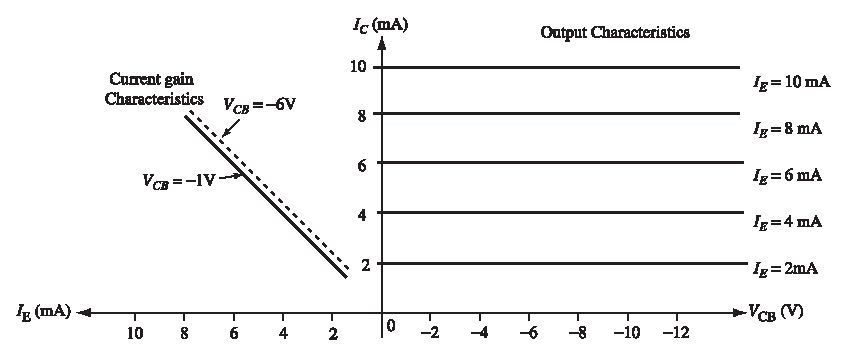
\includegraphics{chap2/S3-EE-03-020.eps}
\caption{Current gain characteristics of common-base configuration}\label{fig3.26}
\end{figure}

Note that the characteristics do not change significantly for variations in $V_{CB}$. Current gain characteristics can also be obtained from the output characteristics. This is illustrated in the example given below.

\begin{example}\label{exam3.13}
Obtain the current gain characteristics for $V_{CB}=-3V$, from the common-base output characteristics shown below.
\begin{figure}[H]
\centering
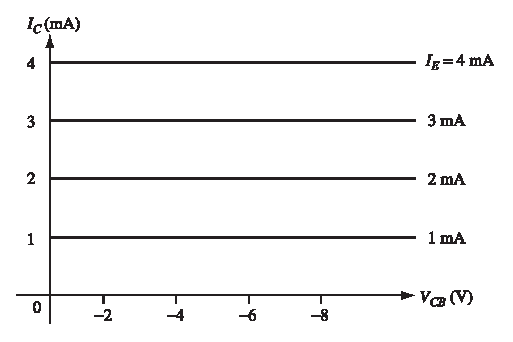
\includegraphics{chap2/S3-EE-03-021.eps}
\end{figure}
\end{example}

\begin{solution}
Draw a vertical line corresponding to $V_{CB}=-3V$ on the output characteristics. Mark the points $P$ and $Q$ where the vertical line intersects the output characteristics. Read off values of $I_{E}$ corresponding to $P$ and $Q$.

\vskip .1cm
At $P$, $I_{C}=1\text{\,mA}$~ and~ $I_{E}=1\text{\,mA}$.

\vskip .1cm
At $Q$, $I_{C}=4\text{\,mA}$~ and~ $I_{E}=4\text{\,mA}$.
\begin{figure}[H]
\centering
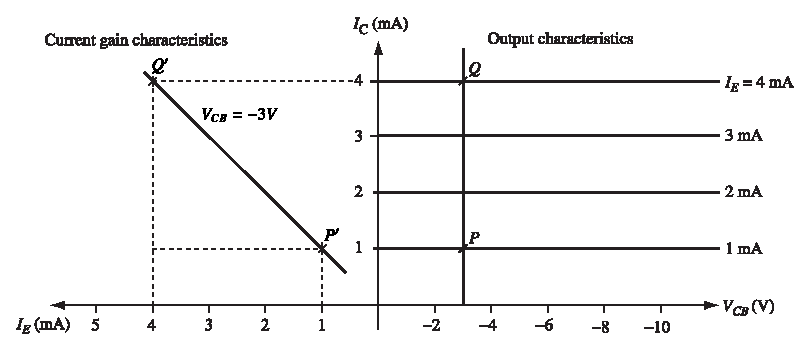
\includegraphics{chap2/S3-EE-03-022.eps}
\end{figure}

Locate the points $P$ and $Q$ on the output characteristics as $P'$ and $Q'$. Join $P'$ and $Q'$ to get the current gain characteristic.
\end{solution}

\begin{example}\label{exam3.14}
Obtain the common-base current gain characteristic for $V_{CB}=-4V$ from the common-base output characteristics shown below.
\begin{figure}[H]
\centering
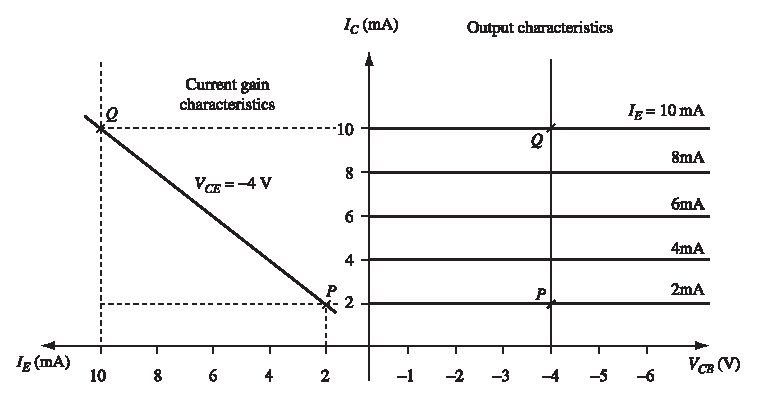
\includegraphics[scale=1.1]{chap2/S3-EE-03-025.eps}
\end{figure}
\end{example}

\begin{solution}
Draw a vertical line at $V_{CB}=-4V$.

\vskip .1cm
Mark points $P$ and $Q$.

\vskip .1cm
$P$ corresponds to $I_{C}=2\text{\,mA}$~ and~ $I_{E}=2\text{\,mA}$.

\vskip .1cm
$Q$ corresponds to $I_{C}=10\text{\,mA}$~ and~ $I_{E}=10\text{\,mA}$.

\vskip .1cm
Locate $P$ and $Q$ on $I_{C}$ versus $I_{E}$ graph.

\vskip .1cm
Joint $PQ$ to get the current gain characteristics.
\end{solution}

\section{Common-Emitter input characteristics}\label{sec3.20}

The common-emitter input characteristics\index{Common-emitter configuration!input characteristics} shows the variation of $I_{B}$ as a function of $V_{BE}$ at the constant $V_{CE}$. The circuit of $npn$ transistor for obtaining common-emitter\index{Transistor characteristics!ce} input characteristics is shown in Fig.~\ref{fig3.27}. $V_{CE}$ is set to a convenient value. $V_{BE}$ is varied in suitable steps and at each step $I_{B}$ value is recorded. The same procedure is repeated for different settings of $V_{CE}$. When these results are plotted, a family of input characteristics is obtained as shown in Fig.~\ref{addfig3.28}.

\smallskip

The following observations are made from the input characteristics of Fig.~\ref{addfig3.28}.
\begin{itemize}
\item
The CE input characteristics resembles the $V$-$I$ characteristics of forward biased $p$-$n$ junction. It is important to note that $I_{B}$ is only a small portion of the total current $I_{E}$ that flows across the forward biased base-emitter junction.

\item
At a constant $V_{BE}$, $I_{B}$ decreases with increase in $V_{CE}$. This is due to the fact that with increase in $V_{CE}$, the depletion region at the reverse biased collector-base junction widens, which reduces the base width. Consequently, more charge carriers from the emitter flow across the collector-base junction and fewer flow out of the base terminal. The reduction in base width due to increase in $V_{CE}$ is called {\em base width modulation} or {\em Early effect}.

\item The input current $I_{B}$ increases less rapidly with increase in input voltage $V_{BE}$. This indicates that input resistance is larger in common-emitter configuration.
\end{itemize}

\begin{figure}[H]
\centering
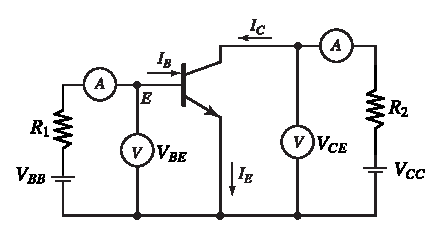
\includegraphics[scale=1.1]{chap2/S3-EE-03-027.eps}
\smallskip
\caption{Circuit for determining transistor common-emitter characteristics}\label{fig3.27}
\end{figure}

\newpage

\begin{figure}[H]
\centering
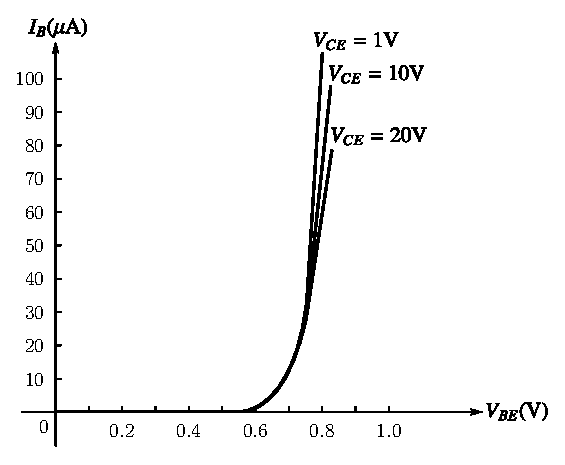
\includegraphics{chap2/S3-EE-03-028.eps}
\caption{The common-emitter input characteristics}\label{addfig3.28}
\end{figure}

\section{Common-Emitter output characteristics}\label{sec3.21}

The common-emitter output characteristics\index{Common-emitter configuration!output characteristics} shows the variation of $I_{C}$ as a function of $V_{CE}$ at a constant $I_{B}$. The circuit for obtaining common-emitter output characteristics is shown in Fig.~\ref{fig3.27}. $I_{B}$ is set to a convenient value, $V_{CE}$ is varied in suitable steps and at each step $I_{C}$ value is recorded. The same procedure is repeated for different settings of $I_{B}$. When these results are plotted a family of output characteristics is obtained as shown in Fig.~\ref{fig3.29}.

The following observations are made from the characteristics of Fig.~\ref{fig3.29}.
\begin{itemize}
\item
With increase in $V_{CE}$, the base width decreases due to increase in the depletion width of collector-base junction. Therefore more charge carriers are drawn from the emitter to the collector. Thus $I_{C}$ increases to some extent with increase in $V_{CE}$ although $I_{B}$ is held constant. As a result the slopes of the common-emitter output characteristics are much more pronounced than those of common-base characteristics.


\item Output characteristics in common-emitter configuration has some slope while common-base configuration has almost horizontal characteristics. This indicates that output resistance of common-emitter configuration is less than that of common-base configuration.

\item The input current $I_{B}$ is in micro-amperes and the output current $I_{C}$ is in milli-ampers. Hence the current gain in common-emitter configuration is large.
\begin{figure}[H]
\centering
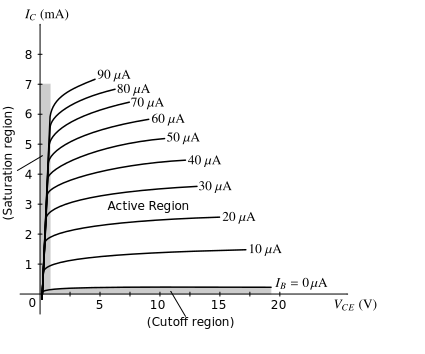
\includegraphics{chap2/S3-EE-03-029.eps}
\caption{The common-emitter output characteristics}\label{fig3.29}
\end{figure}

\item Applying Kirchhoff's Voltage Law to the transistor shown in Fig.~\ref{fig3.30} we have 
$$
V_{CE}-V_{BE}-V_{CB}=0 \ \Rightarrow \ V_{CB}=V_{CE}-V_{BE}
$$
\begin{figure}[H]
\centering
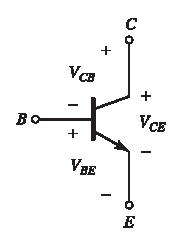
\includegraphics{chap2/S3-EE-03-030.eps}
\caption{Voltage polarities in $npn$ transistor}\label{fig3.30}
\end{figure}

\eject

\item At the knee of the characteristics, $V_{CE}$ is small. When $V_{CE}=V_{BE}$, $V_{CB}=0$ i.e., no reverse bias on collector-base junction. Therefore with decrease in $V_{CE}$, $V_{CB}$ decreases and hence $I_{C}$ decreases. Further reduction in $V_{CE}$ causes the collector-base junction to be forward biased. The forward bias repels the charge carriers injected from the emitter, thus reducing $I_{C}$ to zero.

\item The region of characteristics very close to $I_{C}$ axis where $V_{CE}$ is small is the saturation region. {\em In saturation region both emitter-base and collector-base junctions are forward biased.}

\item The region of characteristics below the output characteristic curve corresponding to $I_{B}=0$ is the cut-off region. {\em In cut-off region both the junctions are reverse biased.}

\item The region to the right of saturation region and above the cut-off region is the active region. In active region emitter-base junction is forward biased and collector-base junction is reverse biased.
\end{itemize}

If $V_{CE}$ exceeds a maximum safe level $I_{C}$ increases rapidly and the device may be destroyed due to punch-through.

\section{Current gain characteristics of Common-Emitter configuration}\label{sec3.22}

\vskip -.3cm

\begin{figure}[H]
\centering
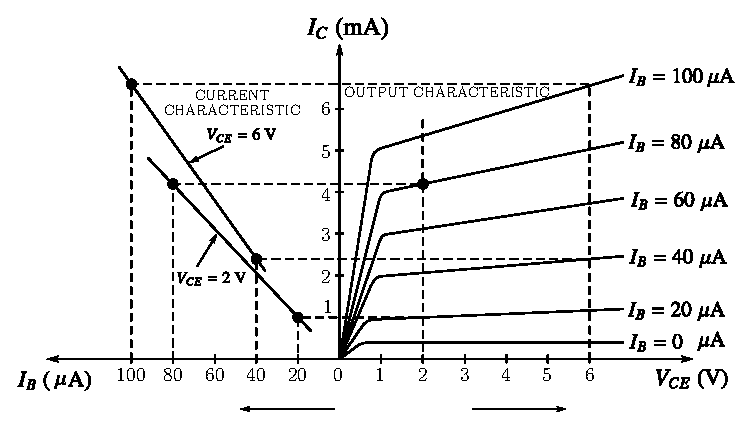
\includegraphics[scale=.95]{chap2/S3-EE-03-031.eps}
\caption{Current gain characteristics of common-emitter configuration}\label{fig3.31}
\end{figure}

\vfill\eject

Common-emitter current gain characteristic\index{Common-emitter configuration!current gain characteristic} shows the variation of $I_{C}$ as a function of $I_{B}$ at constant $V_{CE}$. Current gain characteristics are obtained experimentally by the use of the circuit shown in Fig.~\ref{fig3.27}. $V_{CE}$ is held at a convenient level and $I_{B}$ is varied in suitable steps and at each step $I_{C}$ value is recorded. $I_{C}$ is then plotted as a function of $I_{B}$.

Common-emitter current gain characteristics can be derived from common-emitter output characteristics as shown in Fig.~\ref{fig3.31}. A vertical line is drawn through a selected $V_{CE}$ value and the corresponding levels of $I_{C}$ and $I_{B}$ are read along the line. The $I_{C}$ levels are then plotted as a function of $I_{B}$ and the characteristic is labeled with the $V_{CE}$ used.

\section{Common-Collector input characteristics}\label{sec3.23}

Common-collector input characteristics\index{Common-collector configuration!input characteristics} shows the variation of $I_{B}$ with $V_{BC}$ at a constant $V_{EC}$. The circuit of a $pnp$ transistor for obtaining common-collector\index{Transistor characteristics!cc} input characteristics is shown in Fig.~\ref{fig3.32}.
\begin{figure}[H]
\centering
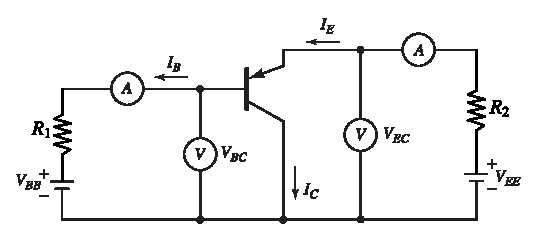
\includegraphics[scale=1.05]{chap2/S3-EE-03-032.eps}
\caption{Circuit for obtaining common-collector input characteristics}\label{fig3.32}
\end{figure}
\begin{itemize}
\item 
$V_{EC}$ is set to a convenient value. $V_{BC}$ is varied in suitable steps and at each step $I_{B}$ value is recorded. The same procedure is repeated for different settings of $V_{EC}$. When these results are plotted a family of input characteristics is obtained as shown in Fig.~\ref{fig3.33}.
\begin{figure}[H]
\centering
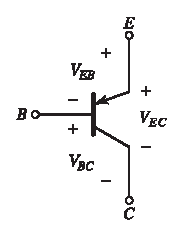
\includegraphics[scale=.95]{chap2/Addfig2.29.eps}
\end{figure}

\itemsep=0pt
\item Applying KVL around the transistor we have
$$
V_{BC}+V_{EB}-V_{EC}=0 \ \ \Rightarrow \ \ V_{BC}=V_{EC}-V_{EB}
$$

\item
Note that the input voltage $V_{BC}$ is largely determined by the $V_{EC}$ level. Since $V_{EC}$ is held constant, $V_{BC}$ also remains constant. Thus input characteristic curves are almost vertical to $V_{BC}$ axis.

\item The above equation can also be written as
$$
V_{EB}=V_{EC}-V_{BC}
$$

At a constant $V_{EC}$, if $V_{BC}$ is increased, $V_{EB}$ reduces and as a result $I_{B}$ decreases.
\begin{figure}[H]
\centering
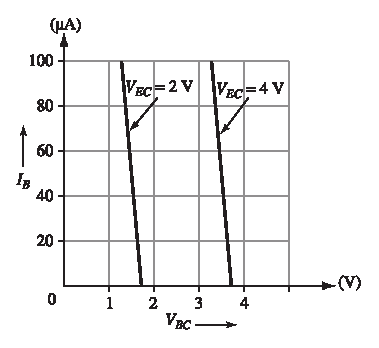
\includegraphics[scale=1.05]{chap2/S3-EE-03-033a.eps}
\caption{Common-collector input characteristics}\label{fig3.33}
\end{figure}
\end{itemize}

\section{Common-Collector output characteristics}\label{sec3.24}

Common-collector output characteristics\index{Common-collector configuration!output characteristics} shows the variation of $I_{E}$ as a function of $V_{EC}$ at a constant $I_{B}$. The circuit for obtaining common-collector output characteristics for a $pnp$ transistor is shown in Fig.~\ref{fig3.32}. $I_{B}$ is set to a convenient value. $V_{EC}$ is varied in suitable steps and at each step $I_{E}$ value is recorded. The same procedure is repeated for different settings of $I_{B}$. When these results are plotted a family of output characteristics is obtained as shown in Fig.~\ref{fig3.34}.


With increase in $V_{EC}$, the base width decreases due to increase in the depletion width of collector-base junction. Therefore more charge carriers are injected from the emitter into the base causing an increase in the emitter current. Since the emitter and collector currents are approximately equal, the common-collector output characteristics are identical to those of common-emitter configuration.
\begin{figure}[H]
\centering
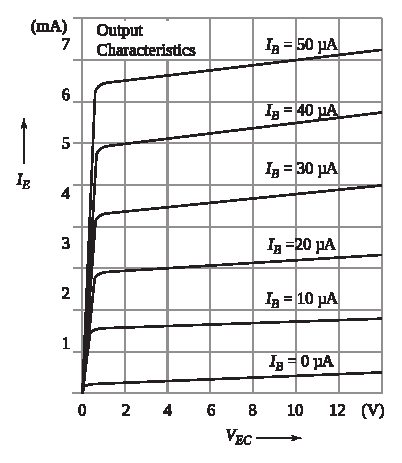
\includegraphics[scale=.88]{chap2/S3-EE-03-033b.eps}
\caption{Common-collector output characteristics}\label{fig3.34}
\end{figure}

\section{Common-Collector current gain characteristics}\label{sec3.25}
\vskip -.5cm
\begin{figure}[H]
\centering
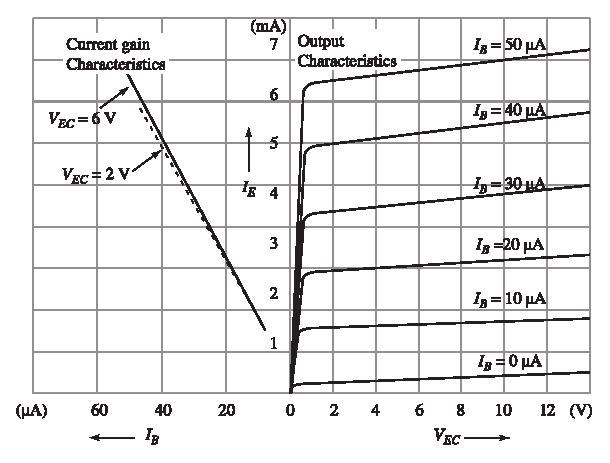
\includegraphics[scale=.88]{chap2/S3-EE-03-034.eps}
\caption{Common collector current gain characteristics}\label{fig3.35}
\end{figure}

\vfill\eject

Fig.~\ref{fig3.35} shows the common-collector current gain characteristics\index{Common-collector configuration!current gain characteristics} which are the plots of $I_{E}$ versus $I_{B}$ for various constant values of $V_{EC}$. They can be obtained experimentally or derived from the output characteristics. Observe that for a given value of base current $I_{B}$ the emitter current $I_{E}$ marginally increases with increase in $V_{EC}$.

\section{Performance comparison of transistor configurations}
\index{Transistor configurations!comparison}

Table~\ref{tab3.1} compares the performace parameters of all the three transistor configurations.

\begin{table}[H]
\centering
\renewcommand{\arraystretch}{1.2}
\caption{Comparison between transistor configurations}\label{tab3.1}
\begin{tabular}{|l|c|c|c|}
\hline
\multirow{2}{*}{\bf Characteristics} & \multicolumn{3}{c|}{\bf Configuration}\\
\cline{2-4}
 & {\bf Common Base} & {\bf Common Emitter} & {\bf Common Collector}\\
\hline
Input impedance & Low & Medium & Very high\\
\hline
Output impedance & Very high & High & Low\\
\hline
Current gain & $\approx 1$ & High & High\\
\hline
Voltage gain & High & High & $\approx\,1$\\
\hline
\multicolumn{1}{|>{\raggedright}p{2.8cm}|}{Phase relation between input and output voltages} & Inphase & $180^{\circ}$\,out of phase & Inphase\\
\hline
Applications & \multicolumn{1}{>{\raggedright}p{3.2cm}|}{Communication systems to amplify high frequency signals} & \multicolumn{1}{>{\raggedright}p{3.2cm}|}{Voltage and current amplification at audio frequencies} & \multicolumn{1}{>{\raggedright}p{3.2cm}|}{Impedance matching}\\
\hline
\end{tabular}
\end{table}

\bigskip
\medskip
\begin{center}
\rule{5cm}{1pt}\\[-2pt]
{\bf Exercise Problems}\\[-4pt]
\rule{5cm}{1pt}
\end{center}

\begin{enumerate}
\renewcommand{\labelenumi}{\bf\theenumi.}
\item Calculate $I_{C}$, $I_{E}$ and $\beta_{dc}$ of a transistor with
$$
\alpha_{dc}=0.97\quad\text{and}\quad I_{B}=100\mu\text{A}
$$

\item Given that $I_{C}=3\text{mA}$ and $I_{E}=3.02$mA calculate $\alpha_{dc}$, $\beta_{dc}$ and $I_{B}$.

\eject

\item A transistor circuit has $I_{C}=5\text{mA}$ and $I_{B}=0.05\text{mA}$
\begin{itemize}
\item[(a)] Calculate $I_{E}$, $\alpha_{dc}$ and $\beta_{dc}$.

\item[(b)] Find the new $I_{B}$ for an $I_{C}$ of 12mA
\end{itemize}

\item A certain transistor circuit has $I_{C}=10\text{mA}$ and $I_{E}=10.04\text{mA}$.
\begin{itemize}
\item[(a)] Calculate $I_{B}$ and $\beta_{dc}$

\item[(b)] Find new $I_{C}$ and $I_{E}$ for the same base current if the transistor is replaced with a transistor of $\beta_{dc}=50$
\end{itemize}

\item Given that $\alpha_{dc}=0.98$, $I_{CB0}=20\text{nA}$, $I_{B}=20\mu\text{A}$. Calculate $I_{C}$ and $I_{E}$.

\item Calculate the voltage gain of a transistor circuit given the following data.
\begin{align*}
& \beta_{dc}=100\qquad R_{C}=5k\Omega\\[3pt]
& \pm V_{BE}=\pm 60\text{mV}\qquad \pm \Delta I_{B}=\pm 15\mu\text{A}
\end{align*}

\end{enumerate}
